\documentclass[tikz,border=12pt]{standalone}
\usepackage[T1]{fontenc}
\usepackage{mathpazo}
\usepackage{amsmath,amssymb}
\usetikzlibrary{arrows.meta, positioning, calc, fit, patterns, decorations.pathreplacing}

\definecolor{stblue}{HTML}{7B97AD}
\definecolor{rwgold}{HTML}{B8995E}
\definecolor{sage}{HTML}{7A9A7E}
\definecolor{dkbrown}{HTML}{3D3530}
\definecolor{wmgray}{HTML}{7B7067}
\definecolor{cream}{HTML}{F9F6F0}
\definecolor{border}{HTML}{D4C9B8}
\definecolor{terracotta}{HTML}{C47A6A}
\definecolor{lavender}{HTML}{907EA0}

\begin{document}
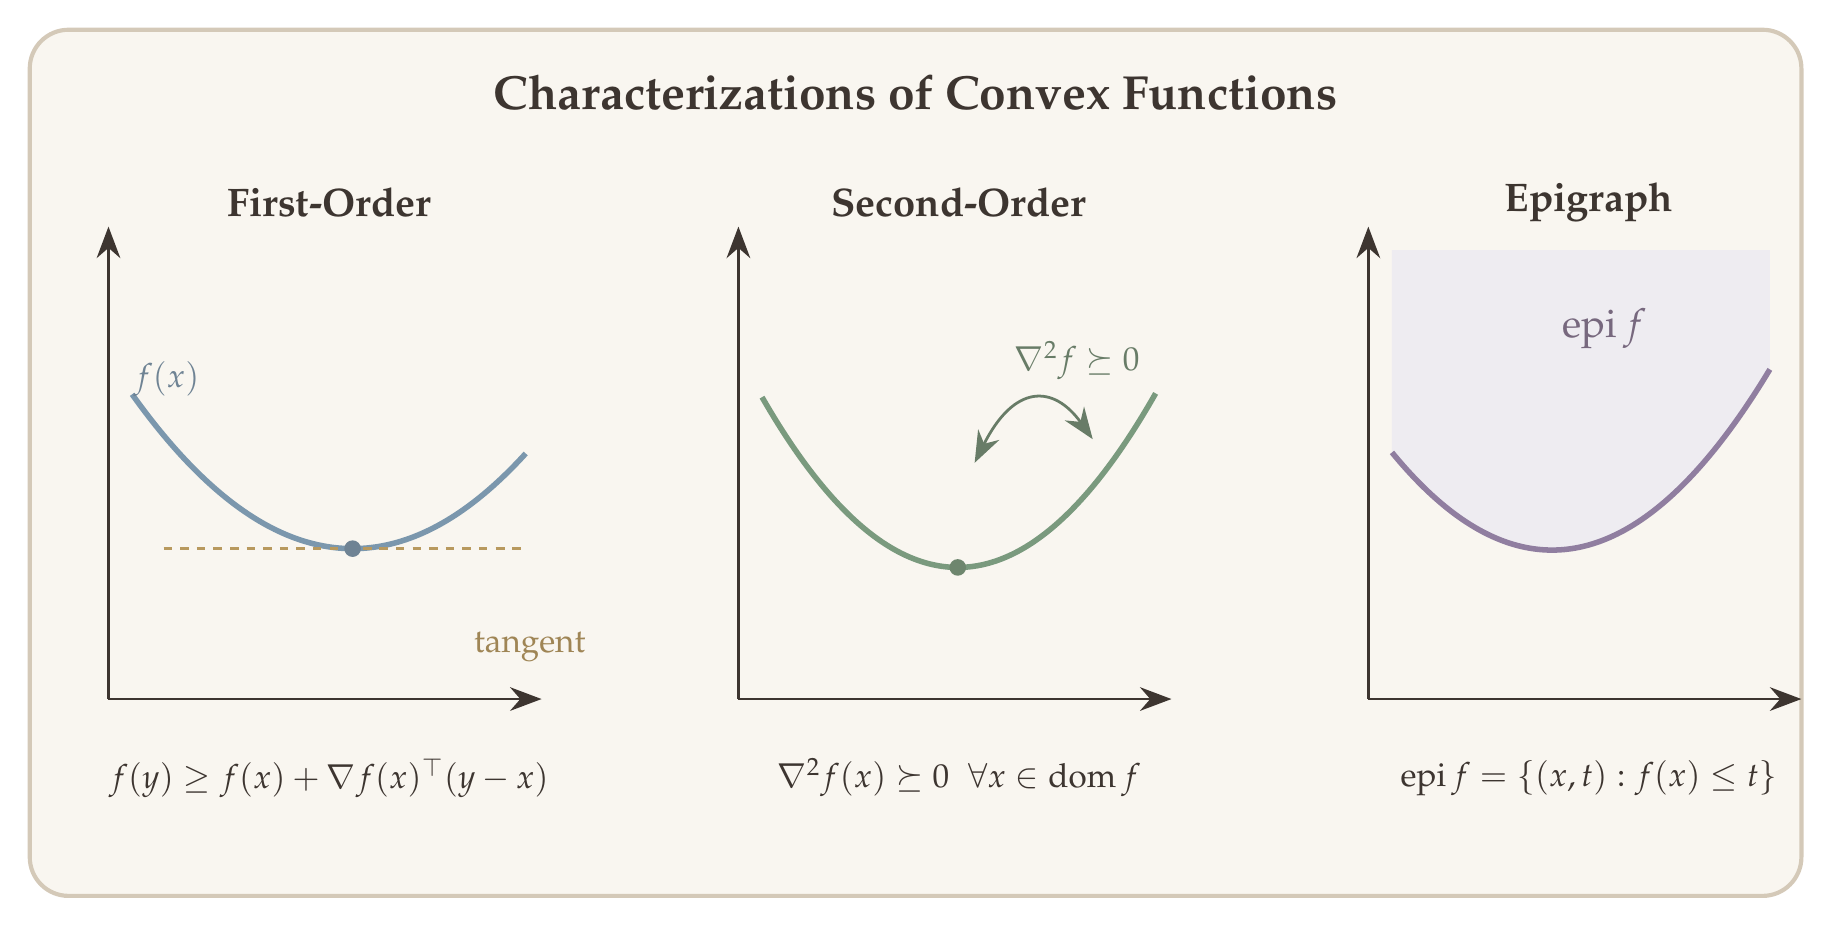
\begin{tikzpicture}[>={Stealth[length=4mm, width=3mm]}, line width=1.5pt]

% Background
\fill[cream, rounded corners=14pt] (-0.5,-3.5) rectangle (22,7.5);
\draw[border, line width=1.5pt, rounded corners=14pt] (-0.5,-3.5) rectangle (22,7.5);

% Title
\node[font=\LARGE\bfseries, text=dkbrown] at (10.75,6.7) {Characterizations of Convex Functions};

% ========== Panel 1: First-order condition ==========
\begin{scope}[shift={(3,1.5)}]
  % Axes
  \draw[->, dkbrown, line width=1pt] (-2.5,-2.5) -- (3,-2.5);
  \draw[->, dkbrown, line width=1pt] (-2.5,-2.5) -- (-2.5,3.5);

  % Convex function
  \draw[stblue, line width=2pt, smooth, domain=-2.2:2.8, samples=100]
    plot (\x, {0.25*\x*\x - 0.3*\x - 0.5});

  % Tangent line at x=0.6
  \pgfmathsetmacro{\tx}{0.6}
  \pgfmathsetmacro{\ty}{0.25*\tx*\tx - 0.3*\tx - 0.5}
  \pgfmathsetmacro{\slope}{0.5*\tx - 0.3}
  \draw[rwgold, line width=1.2pt, dashed, domain=-1.8:2.8, samples=50]
    plot (\x, {\ty + \slope*(\x - \tx)});

  % Point on curve
  \fill[stblue!80!dkbrown] (\tx, \ty) circle (3pt);

  % Labels
  \node[font=\large, text=stblue!80!dkbrown, above left] at (-1.2,1.2) {$f(x)$};
  \node[font=\large, text=rwgold!80!dkbrown, below right] at (2,-1.5) {tangent};

  % Title and formula
  \node[font=\Large\bfseries, text=dkbrown] at (0.3,3.8) {First-Order};
  \node[font=\large, text=dkbrown] at (0.3,-3.5) {$f(y) \geq f(x) + \nabla f(x)^\top(y - x)$};
\end{scope}

% ========== Panel 2: Second-order condition ==========
\begin{scope}[shift={(11,1.5)}]
  % Axes
  \draw[->, dkbrown, line width=1pt] (-2.5,-2.5) -- (3,-2.5);
  \draw[->, dkbrown, line width=1pt] (-2.5,-2.5) -- (-2.5,3.5);

  % Upward parabola (strong convexity)
  \draw[sage, line width=2pt, smooth, domain=-2.2:2.8, samples=100]
    plot (\x, {0.35*\x*\x - 0.2*\x - 0.8});

  % Curvature annotation
  \draw[sage!70!dkbrown, line width=1pt, <->] (0.5,0.5) .. controls (1,1.5) and (1.5,1.5) .. (2,0.8);
  \node[font=\large, text=sage!70!dkbrown] at (1.8,1.8) {$\nabla^2 f \succeq 0$};

  % Minimum point
  \pgfmathsetmacro{\minx}{0.2/0.7}
  \pgfmathsetmacro{\miny}{0.35*\minx*\minx - 0.2*\minx - 0.8}
  \fill[sage!80!dkbrown] (\minx, \miny) circle (3pt);

  % Title and formula
  \node[font=\Large\bfseries, text=dkbrown] at (0.3,3.8) {Second-Order};
  \node[font=\large, text=dkbrown] at (0.3,-3.5) {$\nabla^2 f(x) \succeq 0 \;\; \forall x \in \mathrm{dom}\, f$};
\end{scope}

% ========== Panel 3: Epigraph ==========
\begin{scope}[shift={(19,1.5)}]
  % Axes
  \draw[->, dkbrown, line width=1pt] (-2.5,-2.5) -- (3,-2.5);
  \draw[->, dkbrown, line width=1pt] (-2.5,-2.5) -- (-2.5,3.5);

  % Shaded epigraph (region above curve)
  \fill[lavender!15] (-2.2,{0.3*(-2.2)*(-2.2) + 0.1*(-2.2) - 0.6})
    plot[smooth, domain=-2.2:2.6, samples=80] (\x, {0.3*\x*\x + 0.1*\x - 0.6})
    -- (2.6,3.2) -- (-2.2,3.2) -- cycle;

  % Function curve
  \draw[lavender, line width=2pt, smooth, domain=-2.2:2.6, samples=100]
    plot (\x, {0.3*\x*\x + 0.1*\x - 0.6});

  % Epigraph label
  \node[font=\Large, text=lavender!70!dkbrown] at (0.5,2.2) {$\mathrm{epi}\, f$};

  % Title and formula
  \node[font=\Large\bfseries, text=dkbrown] at (0.3,3.8) {Epigraph};
  \node[font=\large, text=dkbrown] at (0.3,-3.5) {$\mathrm{epi}\, f = \{(x,t) : f(x) \leq t\}$};
\end{scope}

\end{tikzpicture}
\end{document}
